\documentclass{standalone}
\usepackage{tikz}
\usepackage{ctex,siunitx}
\usepackage{tkz-euclide}
\usepackage{amsmath}
\usetikzlibrary{patterns, calc}
\usetikzlibrary {decorations.pathmorphing, decorations.pathreplacing, decorations.shapes,}
\begin{document}
\small
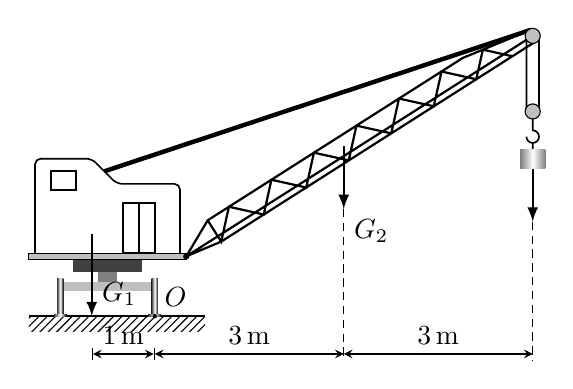
\begin{tikzpicture}[>=stealth,scale=0.8]
  \fill[pattern=north east lines](-2,0)rectangle(0.8,-0.25);
  \draw[thick](-2,0)--(0.8,0);
  \draw[thin,|<->|](-1,-0.6)--(0,-0.6)node[midway,above]{\qty{1}{m}};
  \draw[thin,<->](0,-0.6)--(3,-0.6)node[midway,above]{\qty{3}{m}};
  \draw[thin,<->](3,-0.6)--(6,-0.6)node[midway,above]{\qty{3}{m}};
  \fill[lightgray](-1.5,0.4)rectangle(0,0.55);
  \fill[gray](-0.9,0.7)rectangle(-0.6,0.55);
  \fill[darkgray](-1.3,0.7)rectangle(-0.2,0.9);
  \filldraw[lightgray,draw=black](-2,1.0)rectangle(0.5,0.9);
  \foreach \x in {0,-1.5}
  {
    \fill[left color=darkgray,right color=black,middle color=white](\x-0.05,0)rectangle(\x+0.05,0.6);
    \fill[left color=darkgray,right color=black,middle color=white](\x-0.1,0)rectangle(\x+0.1,0.03);
  }
  \draw[rounded corners=2pt,semithick](-1.9,1.0)--++(0,1.5)--++(0.9,0)--++(0.4,-0.4)--++(1.0,0)--++(0,-1.1);
  \draw[thick,-latex](-1,1.3)--(-1,0)node[above right]{$G_1$};
  \draw[thick,-latex](3,2.7)--++(0,-1)node[below right]{$G_2$};
  \draw[densely dashed](3,1.7)--(3,-0.7)(6,1.5)--(6,-0.7);
  \fill(0.5,0.95)circle(0.05);
  \draw[semithick](-1.65,2.3)rectangle(-1.25,2.0)(-0.5,1.8)rectangle(0,1.0)(-0.25,1.8)--(-0.25,1.0);
  \draw[semithick](6.1,4.45)--(6.1,3.25)(5.9,4.45)--(5.9,3.25)(6,3.25)--(6,2.95)arc(90:-180:0.1)(6,2.75)--(6,2.65);
  \fill(0,0)circle(1pt)node[above right]{$O$};
  \draw[thick,-latex](6,2.5)--++(0,-1);
  \fill[left color=gray,right color=gray,middle color=white](6.2,2.35)rectangle(5.8,2.65);
  \draw[ultra thick](-0.8,2.3)--(5.969,4.545);
  \draw[thick](0.5,0.95)--++(5.5,3.5)
  (6.054,4.366)--(1.055,1.184)--(0.500,0.950)--(0.840,1.522)--(4.889,4.099)--(5.969,4.545)
  (5.678,4.126)--(5.208,4.231)--(5.104,3.761)--(4.552,3.884)--(4.429,3.332)--(3.877,3.455)--(3.754,2.902)--(3.202,3.025)--(3.079,2.473)--(2.527,2.596)--(2.404,2.043)--(1.852,2.166)--(1.730,1.614)--(1.177,1.737)--(1.055,1.184)--(0.840,1.522);
  \filldraw[lightgray,draw=black](6,4.45)circle(0.12)(6,3.25)circle(0.12);
\end{tikzpicture}
\end{document}